\subsection{Results}
\label{subsec:imagelocresults}

Again HOG features are used describe image patches. This time a more dense field
is required because from the image patches classified as \emph{image} the actual
images are to be extracted. For this purpose the page is divided into 10 by 20
blocks each with one cell. Optionally, features are concatenated to incorporate
more information from the region. This results in 9 by 19 concatenated
features in which a feature vector is built op from one HOG feature, the HOG to
its right, its bottom and its right bottom, concatenated into one.

If the preprocessing step of the linear SVM is used, we need to be careful and
avoid overfitting by training the linear SVM on the same data as the structured
SVM is trained on. Therefor, we used two stage validation learning (see figure
\ref{fig:twostage}). In two stage validation, a different subset of
the training data is repeatedly used to train the linear SVM. The resulting SVM
assigns the
confidence score to rest of the training data in order to finally recreate the
whole training data, but now with scores and without the risk of
overfitting\footnote{Note that we do not use Platt scaling to normalize the
scores assigned by these different SVMs. Empirical results show that this does
actually hurts performance a little, even though more one-vs-all and all-vs-all
multi-class SVMs often exclude this step to safe time as well\cite{duan2005best}}.
Finally the linear SVM is trained on the complete dataset to obtain a model
trained with as much data as possible for the final product.
%\todo{several SVMs and the confidence scores can be used?! Could only find:
%\cite{duan2005best} which indicates exactly the opposite}

\begin{figure}
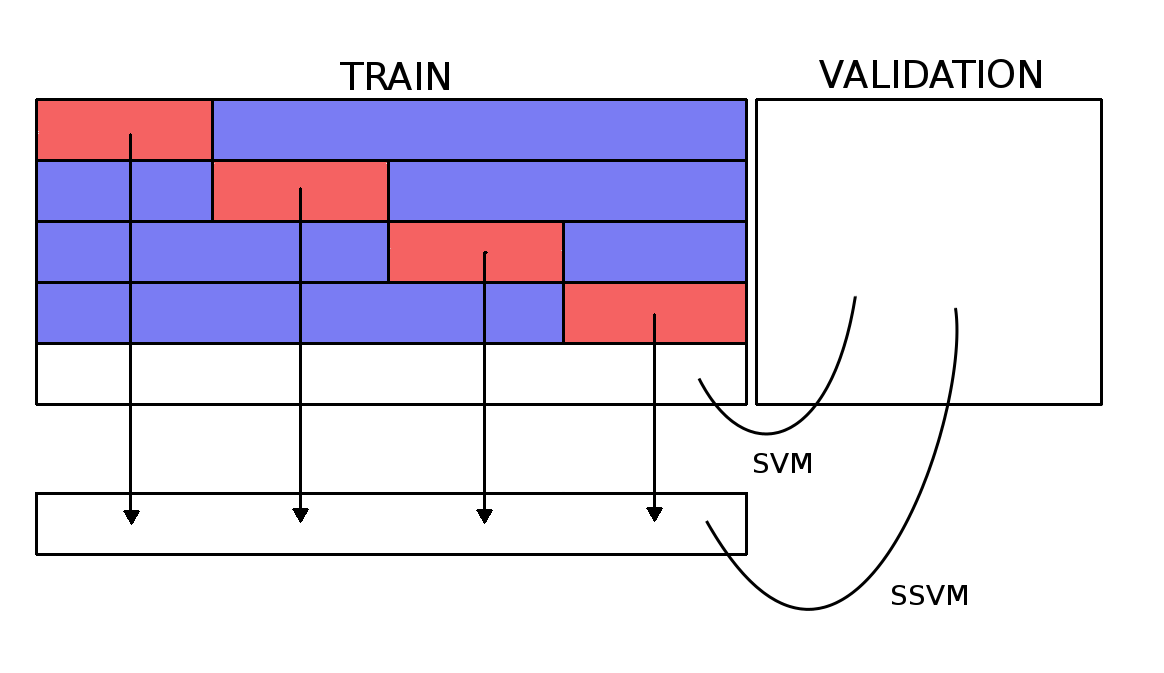
\includegraphics[width=.5\textwidth]{resources/twostage}
\caption{Visualization of two-stage validation training to generate data for the
structured SVM}
\label{fig:twostage}
\end{figure}

We experimented with 4 different settings: directly trained on the structured
SVM and pre-trained with the linear SVM, we then tested both options with the
concatenated features and with the regular features. The same division for the
train, validation and test set has been used as in section \ref{sec:pageclas}.
Tables \ref{tab:imageloccm} and \ref{tab:imagelocresults} show the results for
these settings. The `SVM Only' columns show the results of the
linear SVM for classifying single features. All scores are calculated per
image patch. The true labels are based on the annotated data: whether their centre
is inside or outside a bounding box.

First, the results for the single HOG features in table \ref{tab:imageloccm}.
The extremely low precision indicates that these single HOG features are not
indicative for whether an image patch belongs to an image or text. Presumably, this
large error propagates through to the pre-trained setting, resulting in a low
recall for image patches there as well. The directly trained SSVM was able to
achieve much better results.

\begin{table}
\centering
% Extra colsep creates fancy lines
\begin{tabular}{@{\extracolsep{4pt}}l r r r r r r @{}}
\hline
& \multicolumn{2}{c}{\emph{SVM only}} & \multicolumn{2}{c}{\emph{Pre-trained}} & \multicolumn{2}{c}{\emph{Direct}}
\\\cline{2-3}\cline{4-5}\cline{6-7}
& \textbf{Image} & \textbf{Text} & \textbf{Image} & \textbf{Text} & \textbf{Image} & \textbf{Text} \\
%\textbf{Precision} & 0.099 & 0.973 & 0.271 & 0.979 & 0.271 & 0.979 \\
%\textbf{Recall} & 0.736 & 0.585 & 0.700 & 0.884 & 0.700 & 0.884 \\
%\textbf{F-score} & 0.174 & 0.730 & 0.391 & 0.929 & 0.391 & 0.929\\\hline
%%% NOOOOOO wrooonnggg!
\textbf{Precision} & 0.099 & 0.973 & 0.703 & 0.944 & 0.271 & 0.979 \\
\textbf{Recall}    & 0.736 & 0.585 & 0.040 & 0.999 & 0.700 & 0.884 \\
\textbf{F-score}   & 0.174 & 0.730 & 0.075 & 0.970 & 0.391 & 0.929\\\hline
\end{tabular}
\caption{Results for image localization with single features}
\label{tab:imageloccm}
\end{table}

Secondly, the results for the concatenated features can be found in table
\ref{tab:imagelocresults}. The concatenated features seem to convey more
information about the image patch, as indicated by the rise in precision and
recall for the linear SVM. As a result, the score difference 
in the pre-trained and the directly trained experiments are small, but favor the
pre-trained setting slightly.

\begin{table}
\centering
\begin{tabular}{@{\extracolsep{4pt}}l r r r r r r @{}}
\hline
 & \multicolumn{2}{c}{\emph{SVM Only}}  & \multicolumn{2}{c}{\emph{Pre-trained}} & \multicolumn{2}{c}{\emph{Direct}} \\
 \cline{2-3} \cline{4-5} \cline{6-7}
  & \textbf{Image} & \textbf{Text} & \textbf{Image} & \textbf{Text} & \textbf{Image} & \textbf{Text} \\
\textbf{Precision} & 0.154 & 0.973 & 0.269 & 0.979 & 0.241 & 0.979 \\
\textbf{Recall} & 0.732 & 0.709 & 0.743 & 0.854 &  0.750 & 0.830 \\
\textbf{F-score} & 0.254 & 0.820 & 0.395 & 0.912 & 0.365 & 0.898 \\\hline
\end{tabular}
\caption{scores for image localization with concatenated features}
\label{tab:imagelocresults}
\end{table}

We can deduce that the CRF, solved by the structured SVM improves performance
significantly.


%\begin{table}
%\centering
%% Extra colsep creates fancy lines
%\begin{tabular}{@{\extracolsep{4pt}}l r r r r r r @{}}
%\hline
%& \multicolumn{2}{c}{\emph{SVM only}} & \multicolumn{2}{c}{\emph{Pre-trained}} & \multicolumn{2}{c}{\emph{Direct}}
%\\\cline{2-3}\cline{4-5}\cline{6-7}
%Real\textbackslash Predicted & \textbf{Image} & \textbf{Text} & \textbf{Image} & \textbf{Text} & \textbf{Image} & \textbf{Text} \\
%\textbf{Image} & 24160 & 8844 & 524523 & 58481 & 524759 & 58245 \\
%\textbf{Text} & 133044 & 324380 & 566567 & 5390857 & 577927 & 5379497 \\\hline
%\end{tabular}
%\caption{Confusion Matrix for image localization with concatenated features}
%\label{tab:imageloccm}
%\end{table}


%\begin{table}
%\centering
%% Extra colsep creates fancy lines
%\begin{tabular}{@{\extracolsep{4pt}}l r r r r r r @{}}
%\hline
%& \multicolumn{2}{c}{\emph{SVM only}} & \multicolumn{2}{c}{\emph{Pre-trained}} & \multicolumn{2}{c}{\emph{Direct}}
%\\\cline{2-3}\cline{4-5}\cline{6-7}
%Real\textbackslash Predicted & \textbf{Image} & \textbf{Text} & \textbf{Image} & \textbf{Text} & \textbf{Image} & \textbf{Text} \\
%\textbf{Image} & 24565 & 8800 &  523370 &  59995 & 523370 & 59995 \\
%\textbf{Text} & 224329 & 315906 &  562795 &  5477440 & 562795 & 5477440\\\hline
%\end{tabular}
%\caption{Confusion Matrix for image localization with concatenated features}
%\label{tab:imageloccm}
%\end{table}

%\todo{Explain results, mention that the difference between Pre-trained and
%not pre-trained is bigger with more discriminative features (2x2 HOG in stead of
%1)}

Figure \ref{fig:imagesExtracted} shows some pages from the book `Les six voyages
tavernier ecuyer baron daubonne qu'il fait en turque, en perse, et aux indes,'
by Jean Baptiste Tavernier, written in 1676. The red squares indicate largest
bounding box around the image patches classified as \emph{text}. The pages were
selected on that at least one image patch was classified as text, but otherwise
at random.

